% We’re writing a tech note (SITCOMTN-149) to capture our
% understanding of the state of the system during on-sky commissioning
% campaign with ComCam.  Please use this ticket to capture the work.
%
% From the introduction:
%
% The Vera C. Rubin Observatory on-sky commissioning campaign using
% the Commissioning Camera (ComCam) began on 24 October 2024 and is
% forecasted to continue through mid-December 2024. This interim
% report provides a concise summary of our understanding of the
% integrated system performance based tests and analyses conducted
% during the first weeks of the ComCam on-sky campaign. The emphasis
% is distilling and communicating what we have learned about the
% system. The report is organized into sections to describe major
% activities during the campaign, as well as multiple aspects of the
% demonstrated system and science performance.
%
% Charge:
%
% The groups within the Rubin Observatory project working on each of
% the activities and performance analyses are charged with
% contributing to the relevant sections of the report. The anticipated
% level of detail for the sections ranges from a paragraph up to a
% page or two of text, depending on the current state of
% understanding, with quantitative performance expressed as summary
% statistics, tables, and/or figures.  The objective for this document
% is to summarize the state of knowledge of the system, rather than
% how we got there or “lessons learned”. The sections refer to
% additional supporting documentation, e.g., analysis notebooks, other
% technotes with further detail, as needed. Given the timelines for
% commissioning various aspects of the system, it is natural that some
% sections will have more detail than others.

\subsection{Instrument Signature Removal}
\label{sec:isr}
\newcommand{\czw}[1]{
  \textbf{CZW: }\textcolor{red}{#1}
}
The quality of the instrument signal removal (ISR) has improved during commissioning, as we create and deploy updated calibration products that better represent the \ComCam system.
The following discussion summarizes our current understanding of a variety of features, both expected and newly seen on \ComCam, and presents our expected prognosis of the behavior of the full LSSTCam.

\subsubsection{Phosphorescence}

There are regions on some of the detectors (most visible in R22\_S01, detector=1) which show bright emission, particularly at bluer wavelengths, as shown in \figRef{isr_phosphorescence_example}.
This is believed to be caused by a thin layer of remnant photo-resist from the manufacturing process that remained on the detector surface, and is now permanent due to the subsequent addition of the anti-reflective coating.
In addition to the large areas, there are also discrete point-source-like or cosmic-ray-like defects caused by accumulations of this material.
Adding to the difficulty of mitigating these defects is that this photo-resist is known to be phosphorescent, explaining why these regions are more noticeable in the bluer filters.

The initial studies of this show that these features can continue to emit light up to several minutes after they've been illuminated.
Due to the long duration of these features, we decided to place manual defect masks over the worst regions.
The first of these manual masks takes up about 3.5\% of that detector, smaller than but consistent with estimates that this would create a pixel loss of approximately one amplifier.

\begin{figure}
  \begin{center}
  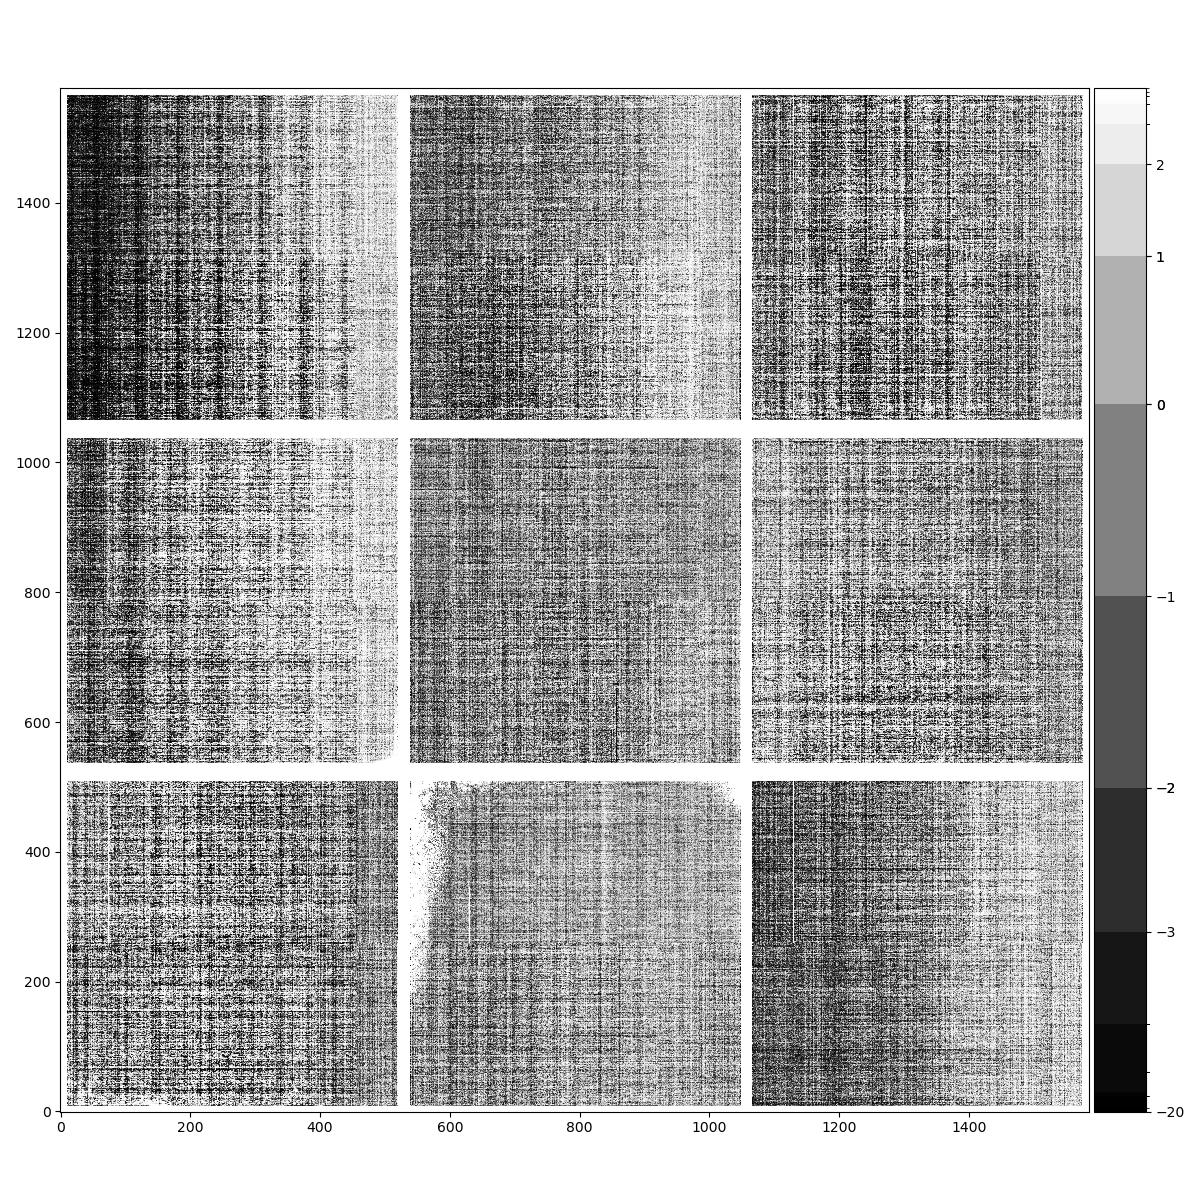
\includegraphics[width=0.5\textwidth]{figures/isr-f01-phosphor_dark_exposure.jpg}
  \caption{The phosphorescence seen in R22\_S01, shown here in a dark exposure taken after a series of twilight flats (exposure=2024112000065).  This material absorbs light at bluer wavelengths and re-emits that energy over a wide range of wavelengths.}
  \label{fig:isr_phosphorescence_example}
  \end{center}
\end{figure}

\begin{figure}
  \begin{center}
  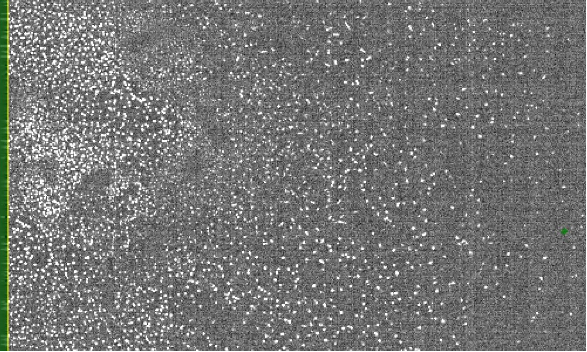
\includegraphics[width=0.8\textwidth]{figures/isr-f02-phosphorescence_point_like.pdf}
  \caption{A full-resolution view of the edge of R22\_S01.  The features shown in this image are point-like sources caused by the trapped phosphorescence photo-resist.}
  \end{center}
\end{figure}

The ITL detectors in LSSTCam are believed to have been cleaned better, so this should be less of an issue on the full camera.

\subsubsection{Vampire pixels}

There are defects on \ComCam that have been classified as ``vampire'' pixels, as they appear as a bright defect with a (generally) axisymmetric region surrounding the bright core, as if the defect is draining charge from its neighbors.
The naming is at least broadly correct, as integrating to large radii shows that these regions do appear to conserve charge.
There is an intensity dependence that makes these vampire pixels different than standard hot pixels, as these pixels do not show up on dark frames, only on flats and science exposures, where the detector surface is illuminated.
After the initial discovery of the bright obvious vampires, we added new masking code that identifies the bright cores that are above 2.0 on the combined flat (pixels that are greater than 200\% of the median flat level), and adds circular masks to the defect list.
This appears to find the most problematic examples, but as we have improved flat quality during commissioning, we are finding that there is a sub-population that are not as severe, but likely have a similar physical mechanism.
This population is still bright on the flat, with peaks around 1.2 (20\% elevated relative to the flat), and may need to be masked as well.
From an initial study in the lab, it appears that all ITL detectors on LSSTCam have a few of these kinds of defects, with two detectors approaching similar contamination levels as R22\_S10 on \ComCam.

\begin{figure}
  \begin{center}
  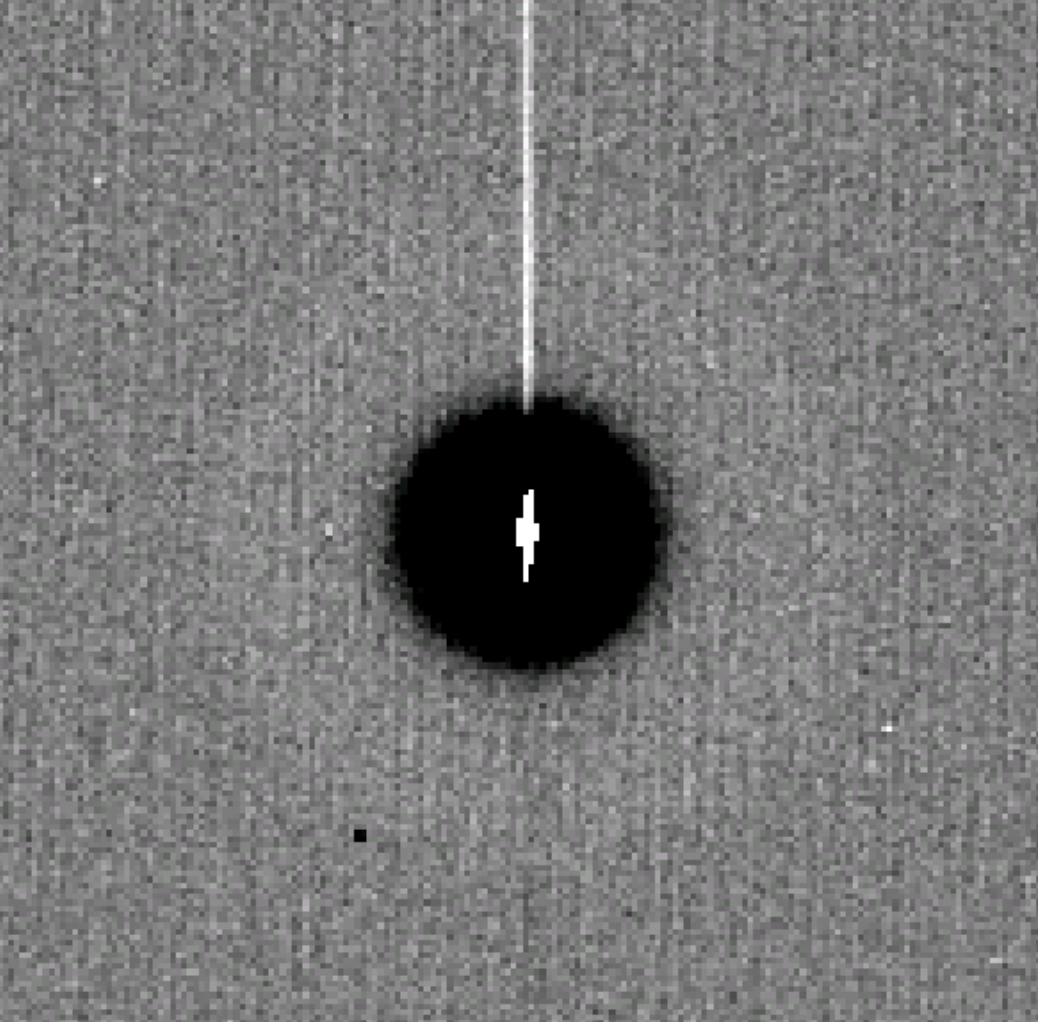
\includegraphics[width=0.5\textwidth]{figures/isr-f03-vampire_pixel.png}
  \caption{A close up of one of the largest vampire pixels.  The bright core and region of depletion are clearly visible.  Currently we only mask the core and depleted region, but will be extending this to mask the persistence-like trail that this feature leaves in the next few weeks.}
  \end{center}
\end{figure}

\begin{figure}
  \begin{center}
  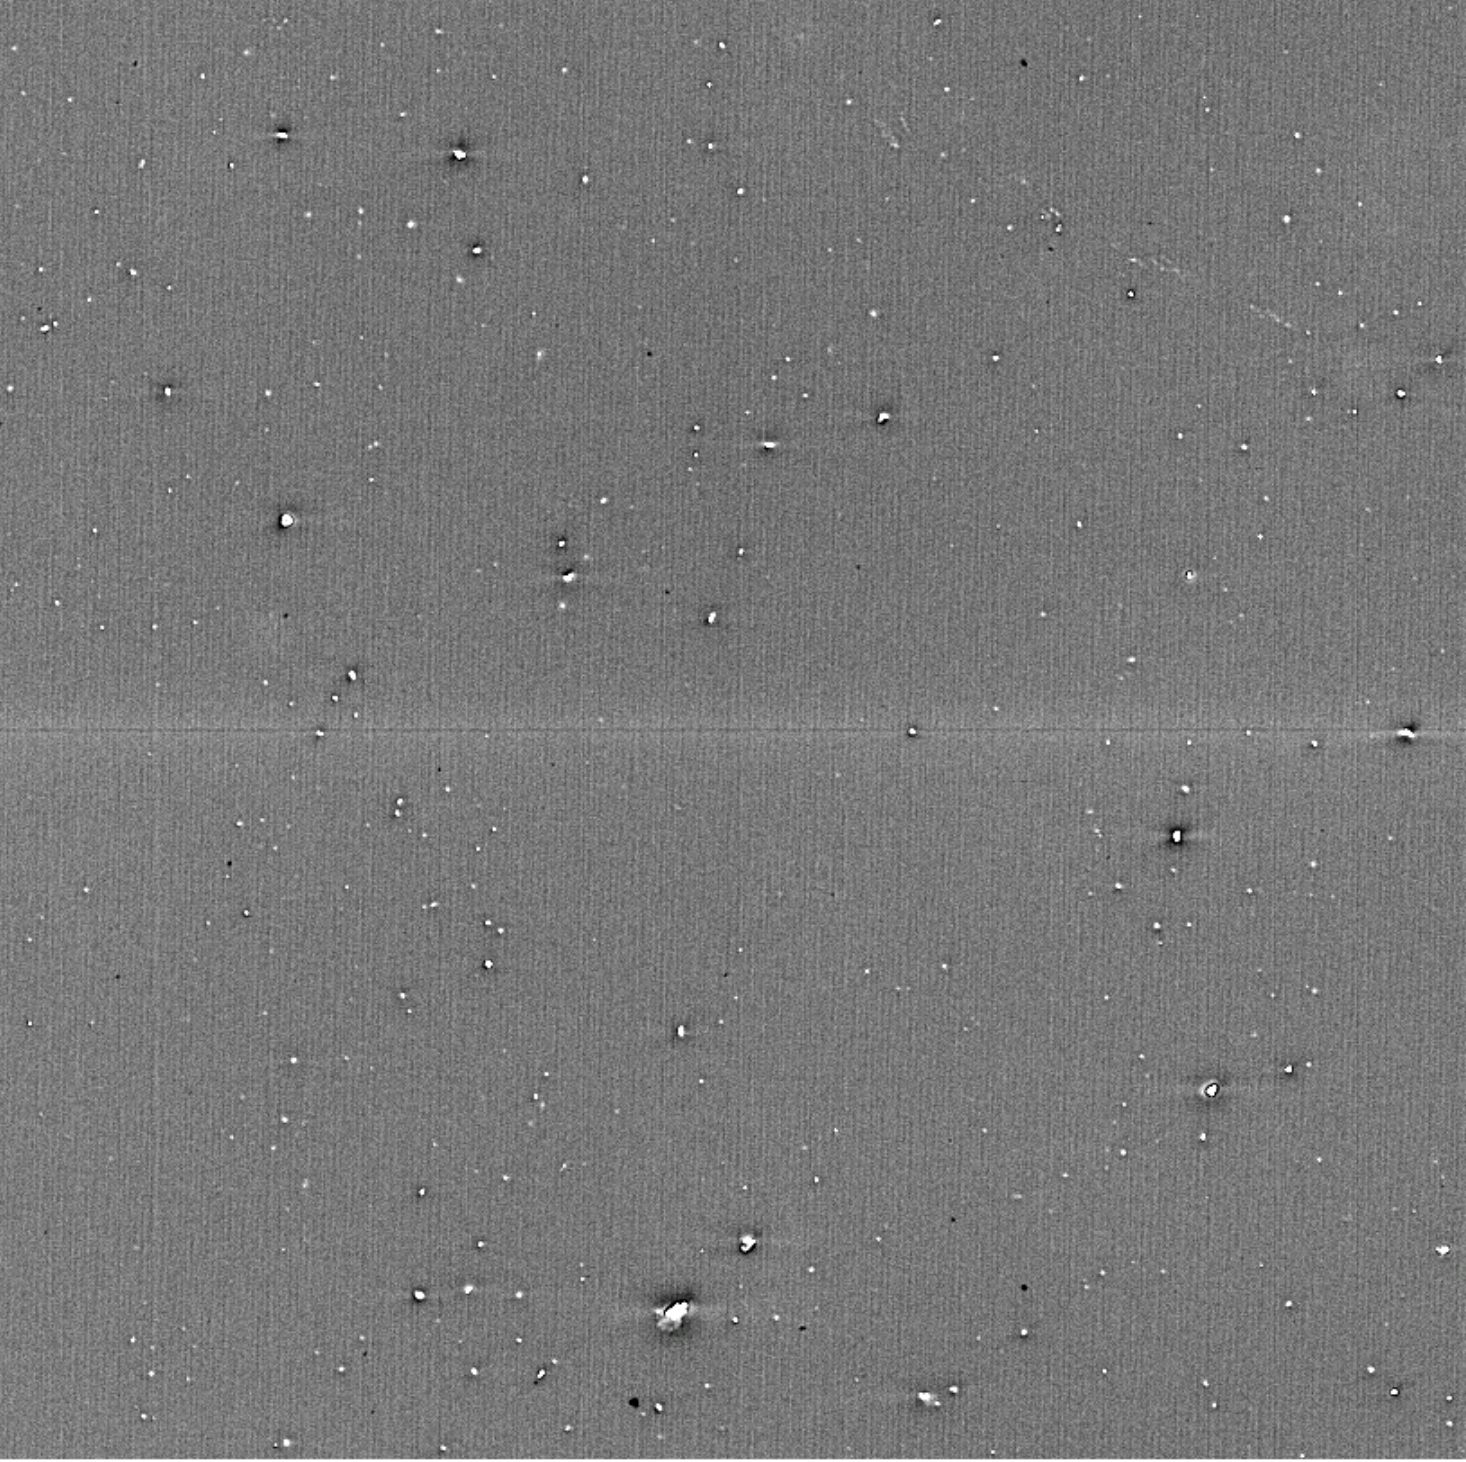
\includegraphics[width=0.5\textwidth]{figures/isr-f04-vampire_pixels_y_det03.png}
  \caption{A view of detector R22\_S10 in y-band, which has a large number of less significant vampire pixels.}
  \end{center}
\end{figure}


\subsubsection{Saturated star effects}

\begin{figure}
  \begin{center}
\linkedFigure{https://rubin-obs.slack.com/files/U0772GZSR8W/F081SU3FAE6/19zqa.png?origin_team=T02SVMGU4&origin_channel=C07RV29CXSR}
    \caption{
      A portion of \texttt{day\_obs 20241127 seq\_num 488} showing the vertical bands which are apparently
        produced by very bright (saturated?) pixels.
    }
\label{fig:darkStreaks}
  \end{center}
\end{figure}

Although we expected to find saturated star trails coming from bright sources, the observed behavior of these trails is unique.
Saturation spikes on most cameras appear as streaks extending from the core of the bright source along the
direction of the parallel transfers, and truncate as the charge bleeds run out of charge (and can no longer
overcome the potentials defining the pixel).
The trails seem with \ComCam, however, extend the entire height of the detectors, crossing the midline break
(as is to be expected in the ITL, but not the E2V, CCDs).
These trails are also not at the expected high state, with the centers of these trails having flux levels
lower than the average sky levels, creating dark trails (See \figRef{darkStreaks}),
On the worst saturated objects, there is also evidence of charge pile-up near the serial register, which can then create fan-like bright features at the edge of the detector.
Those bright features can also then crosstalk onto other amplifiers.

The underlying physics is not well understood. The leading theory is that photo-electrons entering the
$n$-doped channel stops partially cancel the effects of the holes, leading to electric fields which
produce an effect similar to Brighter-Fatter, visible in the background level as well as in objects.
Further study is needed to see if we can correct these trails outside of the regions of charge buildup.
Until we have a correction, we plan to begin masking both the trail and the fan-spread near the serial register.

Although we haven't seen identical features on LATISS (possibly due to the much lower sky levels), the presence of these odd trails on all \ComCam detectors suggests that this is a property of the ITL devices, and so will likely be seen on LSSTCam as well.

\subsubsection{Gain ratios}

\ComCam has been the first large-scale application of the updated ``IsrTaskLSST'' task, which uses a model of how the various signals combine to form the raw images to inform how we correct those signals during the ISR process.
One improvement of this new task is that we now apply per-amplifier gains before flat correction, removing the gain component that was previously included in the flat correction.
This results in the flat containing mainly QE and illumination patterns, which is much ``flatter'' than flats that also include gain terms (which offset the amplifiers relative to each other).


If we have properly diagonalized the flats and the gains, we would expect that applying the gain correction would create images with consistent sky levels across different amplifiers.
However, when we look at images taken on-sky, our initial gain values result in some amplifiers being
significantly different than their neighbors (\figRef{raft_flat_ratio}).
The gains that we use are derived from the photon transfer curve (PTC), which uses flat pairs at different flux levels to monitor the properties of the noise.
We have two of these sequences taken in the lab, and they disagree at the few percent level.
This is similar in scale to the errors necessary to explain the on-sky differences.
Further complicating this issue, the offsets seen in twilight data (used for flats) and that seen during the
night also seem to differ (\figRef{amp_gain_ratios})
These differences so far have not been found to correlate with any device temperature, time, or voltage values.
The gain correction fix appears to be stable, as we've only needed to generate and apply it once.

\begin{figure}
  \begin{center}
  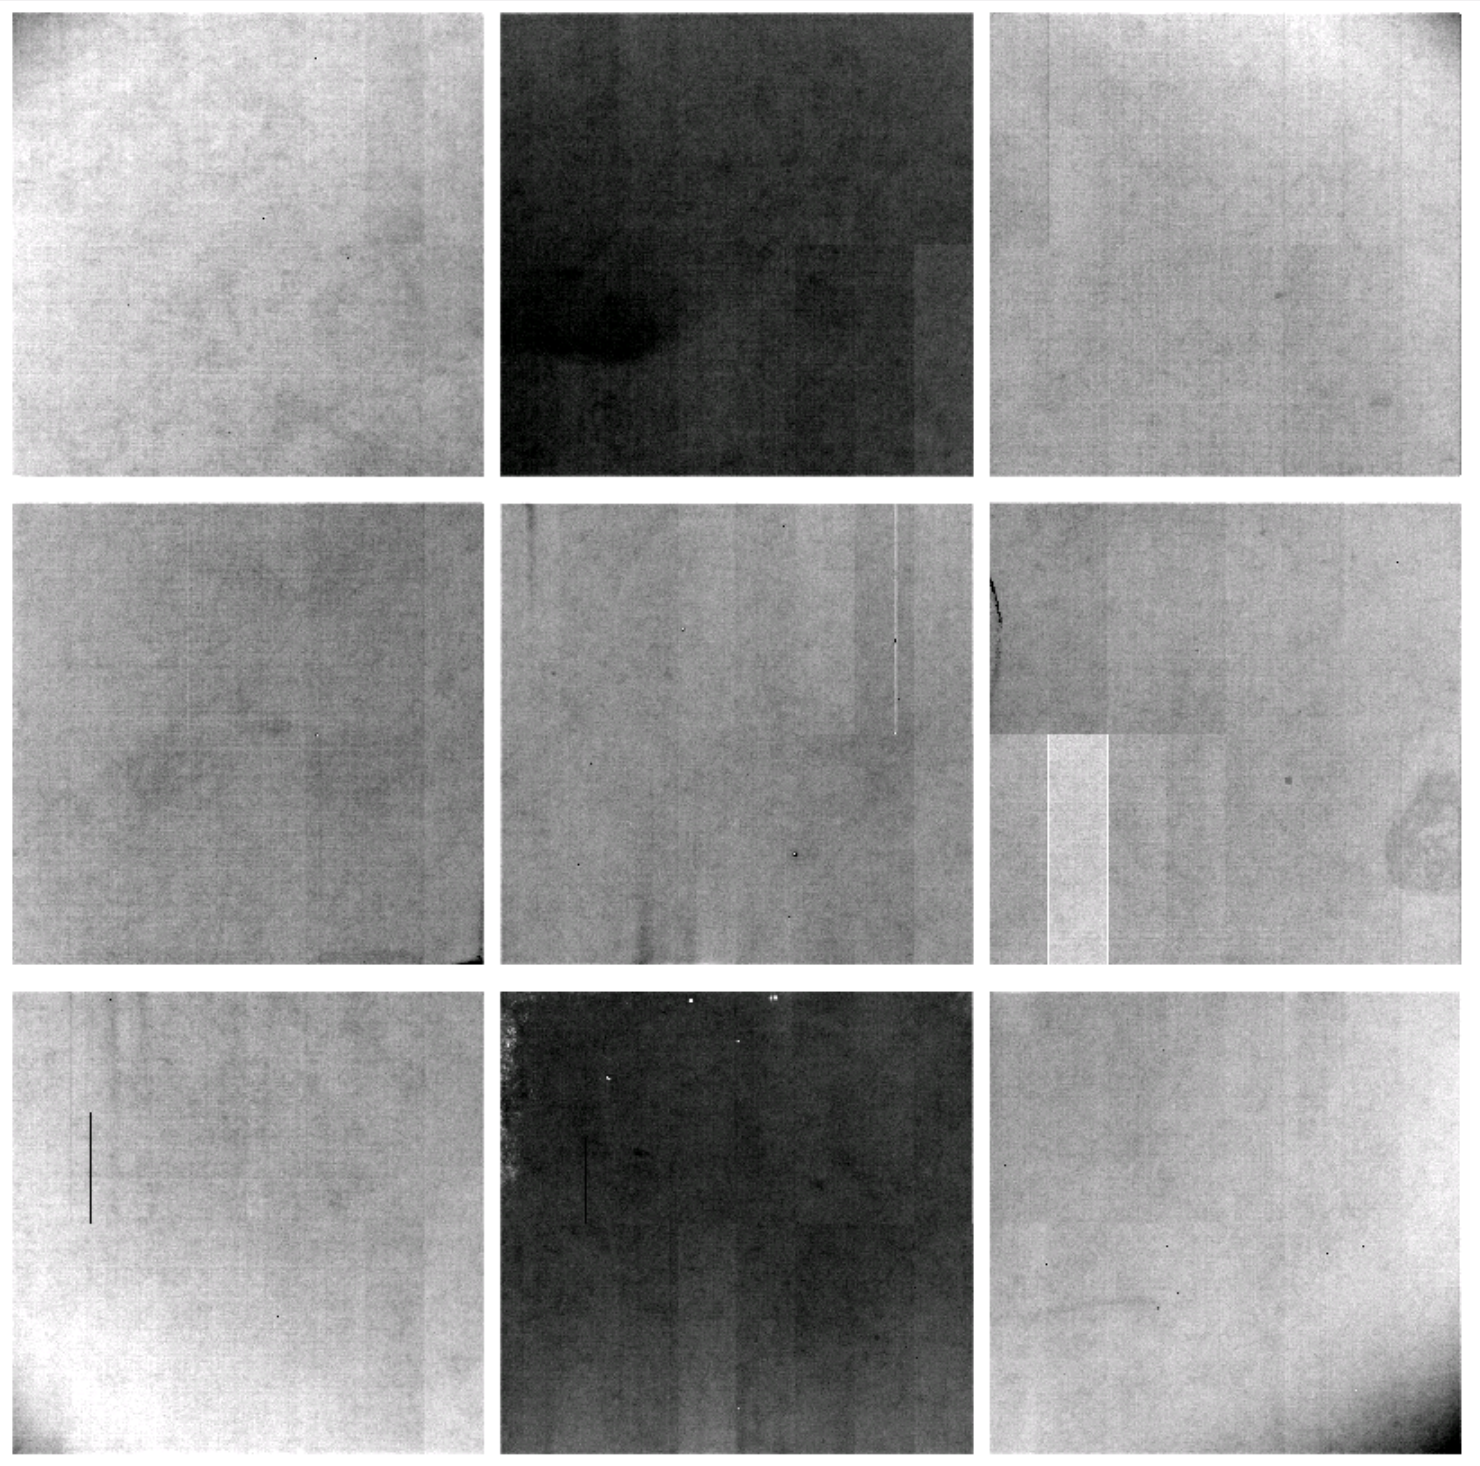
\includegraphics[width=0.5\textwidth]{figures/isr-f06-twilight_flat_ratio.png}
  \caption{The ratio of the twilight-flat divided by a flat constructed from 94 r-band science frames.  The
    scaling ranges from 0.9905 to 1.007.  The visibility of amplifiers is caused by the unknown gain errors.
    The bottom right corner amplifier (C07) on R22\_S21 is one of the indicator amplifiers, as it diverges
    from its neighbors.  Although the C00-C03 amplifiers in R22\_S12 also show significant offsets, these
    amplifiers also have an unrelated CTI issue, making them less reliable indicators.}
  \label{fig:raft_flat_ratio}
  \end{center}
\end{figure}

\begin{figure}
  \begin{center}
  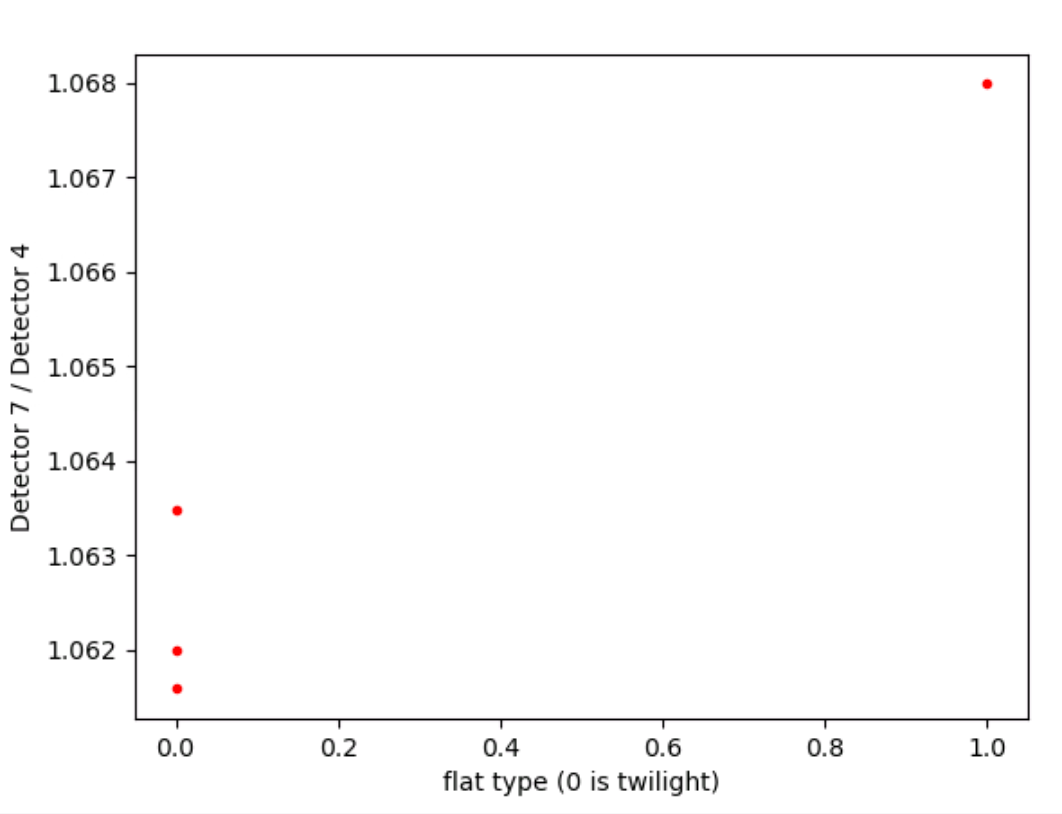
\includegraphics[width=0.5\textwidth]{figures/isr-f05-gain_ratios_by_flat.png}
  \caption{A comparison of the gain ratio between amplifiers in R22\_S12.  C07 is chosen as the indicator amplifier, and C04 is the reference.  We have three twilight flat measurements taken at different rotator angles, and one from the 94 input sky flat.}
  \label{fig:amp_gain_ratios}
  \end{center}
\end{figure}

\subsubsection{Crosstalk}

We are currently using crosstalk values that were constructed by averaging the lab-based ITL measurements taken on LSSTCam.
These are working well, with residuals post correction being only a few electrons peak to peak.
We plan to do a more complete crosstalk study using on-sky data, but the current results suggest that these lab measurements are sufficient for \ComCam, and expect the same to be true for LSSTCam.

\subsubsection{Twilight flats}

Because the flat field screen and illuminator was not available while ComCam was on the telescope, we used dithered, tracked twilight flats to generate the combined flat calibration frames. The exposure time of the twilight flats were dynamically adjusted to hit a target count, generally in the range of 10-20k. The flats taken at a wide range of azimuth angles and rotator angles. See \figRef{twilight_counts} for the counts per pixel per second as a function of sun elevation angle.

This reduction of non-sky signals is imperfect, and an early i-band flat showed a satellite trail as a
result; this was remedied with a more recent flat built using a larger number of exposures.


\begin{figure}
  \centering
  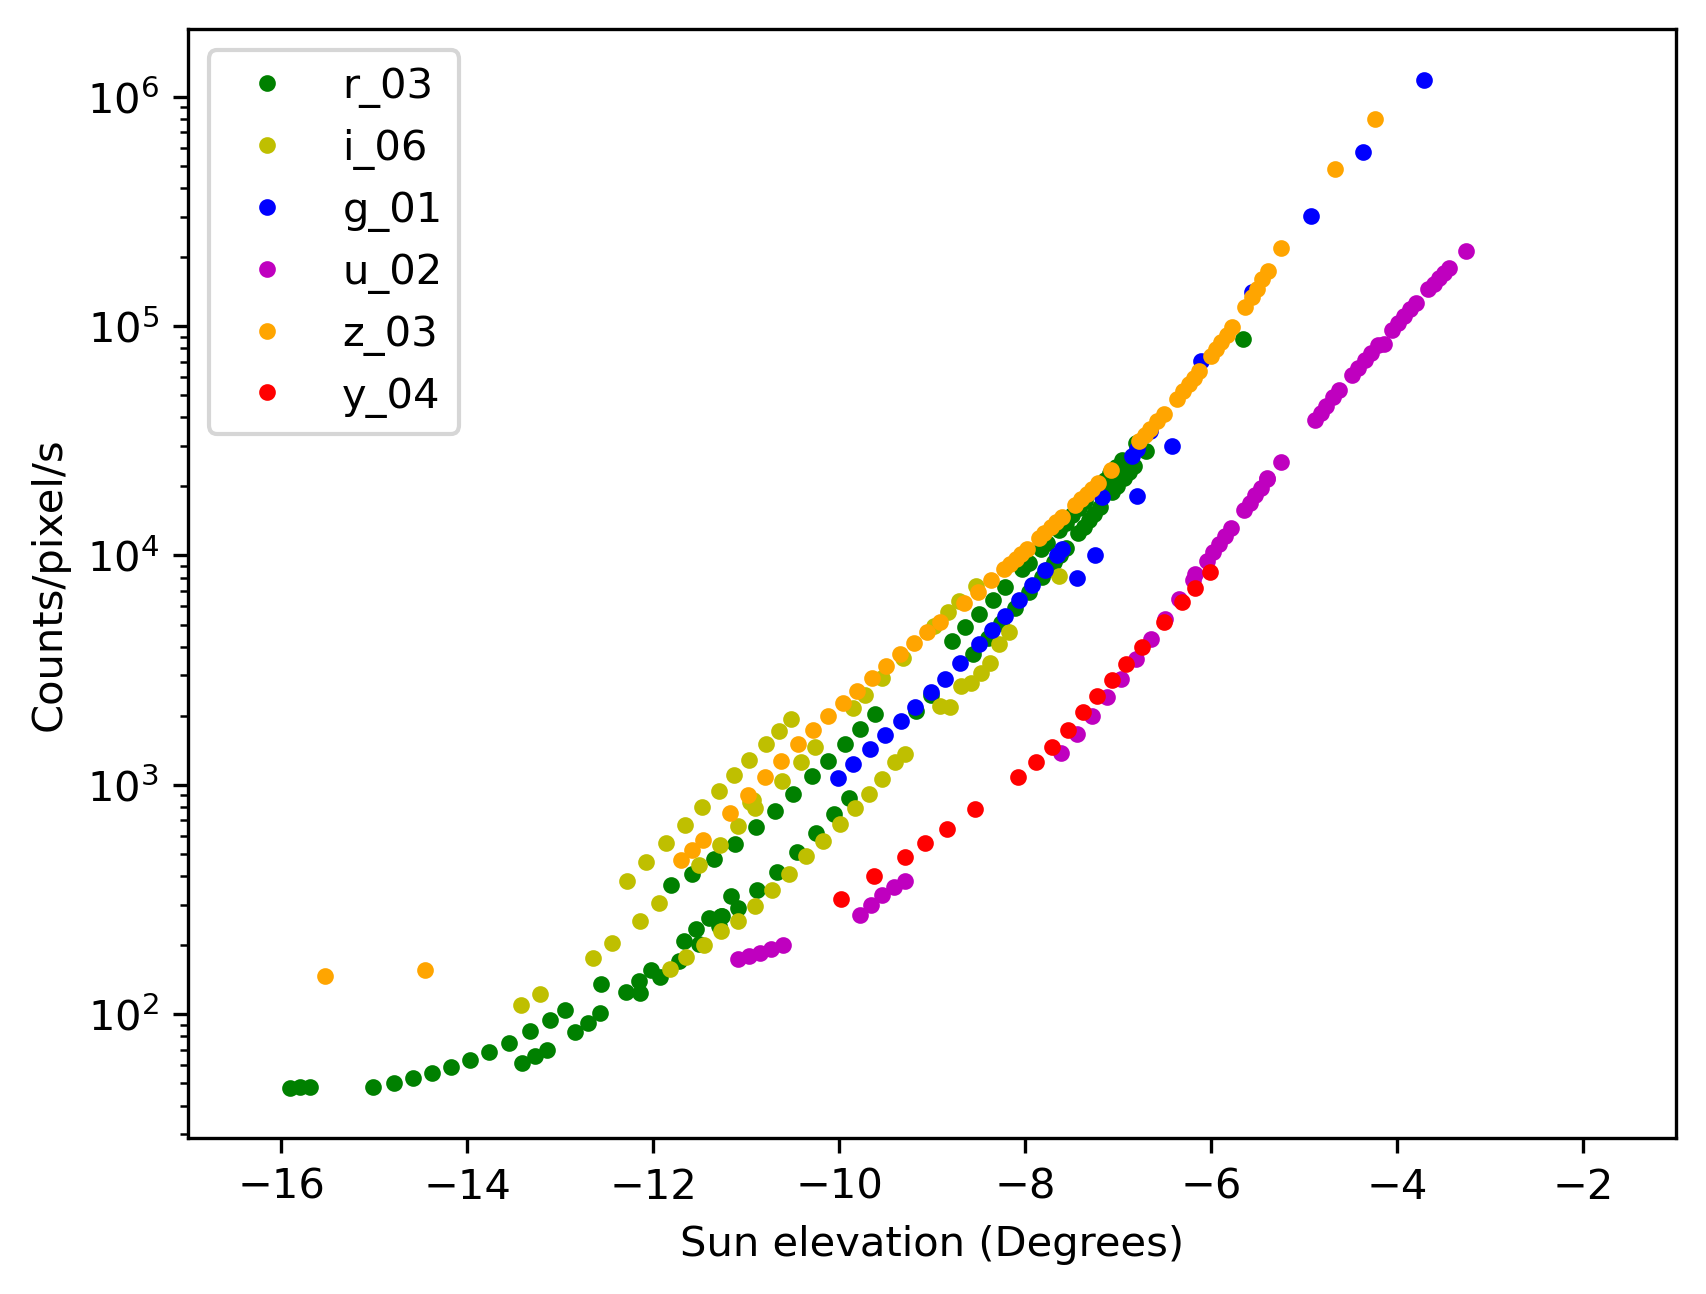
\includegraphics[width=0.5\textwidth]{calibration_data_figures/twilight_flat_counts.png}
  \caption{Twilight flat counts per pixel per second for each filter as a function of sun elevation angle.}
  \label{fig:twilight_counts}
\end{figure}

\subsubsection{Operations}

The Telescope and Auxiliary Instrumentation Calibration Acceptance Board (TAXICAB) has been meeting previously to discuss LATISS calibrations, and has been helping manage calibrations for \ComCam.
This process has not prevented problematic calibrations from being deployed (like the i-band flat with the satellite trail), but it has ensured that multiple people have checked some set of results.
We are generating calibration verification reports regularly as part of this process (available at \url{https://s3df.slac.stanford.edu/people/czw/cpv_reports/}), and plan to add new metrics and checks to these as we discover more features of these detectors.
